Equations \ref{eq: Q1_res} to \ref{eq: w_res} show the ascertained function of the rating curve that was implemented in the script to calculate the perturbed discharge (eq: \ref{eq: Q}), with the transition center $h\_0 = 450$. The coefficient of determination $R^2 = 0.998705$ and the Root Mean Square Error $RMSE = 0.920025$ validate a good fit of the curve (fig: \ref{fig: fitt_curv}). Figure \ref{fig:obs_vs_cal} shows the difference in the calculated discharge values, without any perturbations to the original observed discharge values that were used. The highest peak flow is slightly overestimated as expected from the trend of the rating curve (fig: \ref{fig:obs_vs_cal}). The impact of the variations of the fitting curve to the observed QH-relation is clearly visible in figure \ref{fig:obs_vs_cal} and also confirmed by the residual comparison (fig: \ref{fig:res_comp}, orange line).

\begin{equation}
     \text{Q1(h)} =  1.22871059 \cdot 10^{-4}(h - 25.033145)^{2.1538}
     \label{eq: Q1_res}
\end{equation}

\begin{equation}
     \text{Q2(h)} = 5.83762819\times 10^{-6} (h - 315.640655)^{3.3829}
     \label{eq: Q2_res}
\end{equation}

\begin{equation}
     \text{w(h)} =  \frac{1}{1 + \exp\left(-\frac{h - 450.0000}{6.8602}\right)}\
     \label{eq: w_res}
\end{equation}

\begin{figure}[H]
\centering
  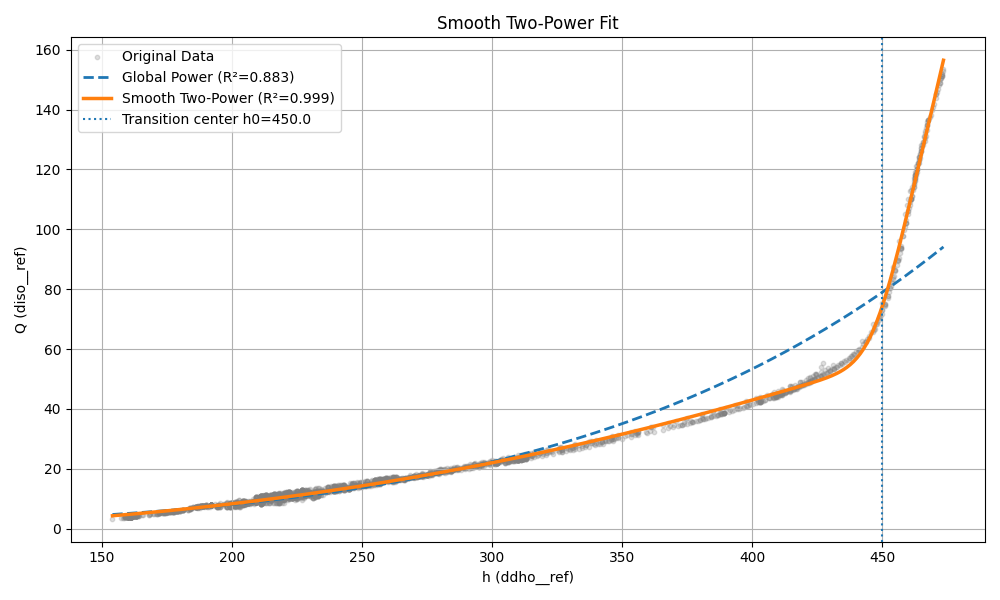
\includegraphics[width=1 \textwidth]{Figures/Ass_05/fitting_curv.png}
    \caption{rating curve}
    \label{fig: fitt_curv}
\end{figure}

\begin{figure}[H]
    \centering
    \begin{minipage}[t]{0.48\textwidth}
        \centering
        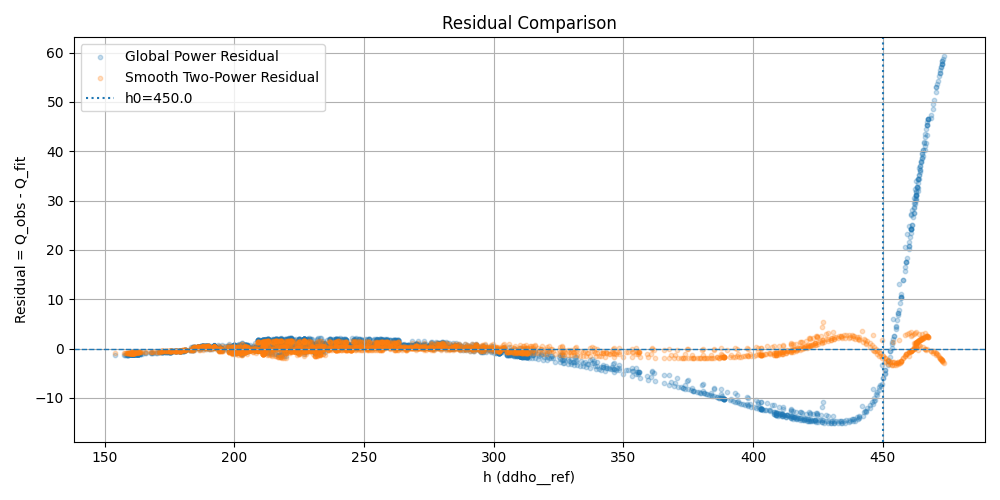
\includegraphics[width=\textwidth]{Figures/Ass_05/fitting_curv_residual_comparison.png}
        \caption{residual comparison}
        \label{fig:res_comp}
    \end{minipage}
    \hfill
    \begin{minipage}[t]{0.48\textwidth}
        \centering
        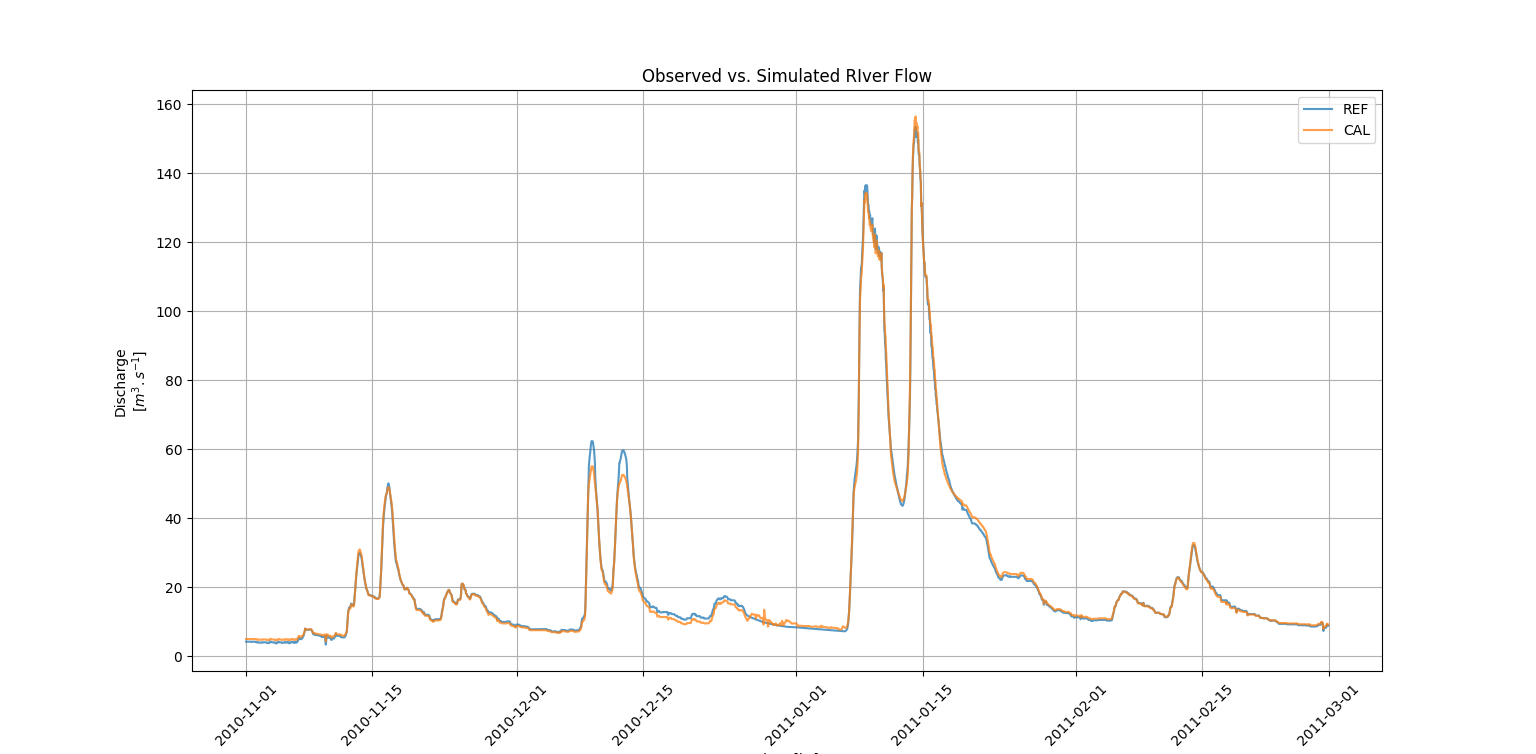
\includegraphics[width=\textwidth]{Figures/Ass_05/obs_vs_cal_diss.png}
        \caption{observed discharge vs calculated}
        \label{fig:obs_vs_cal}
    \end{minipage}
\end{figure}

Regarding the \ac{cdf}, the perturbed discharge follows the shape of the observed \ac{cdf}, with the exception of the high discharges (fig: \ref{fig:cdf}). Since the rating curve holds for water levels above \SI{450}{\text{cm}}, a very steep trend, a large increase in discharge for small changes in water level, was expected. Figure \ref{fig:pert_dis_eg} shows an example of a perturbed discharge. Due to the slight overestimation of the rating curve at very high water levels, this effect is enhanced.  

\begin{figure}[H]
    \centering
    \begin{minipage}[t]{0.48\textwidth}
        \centering
        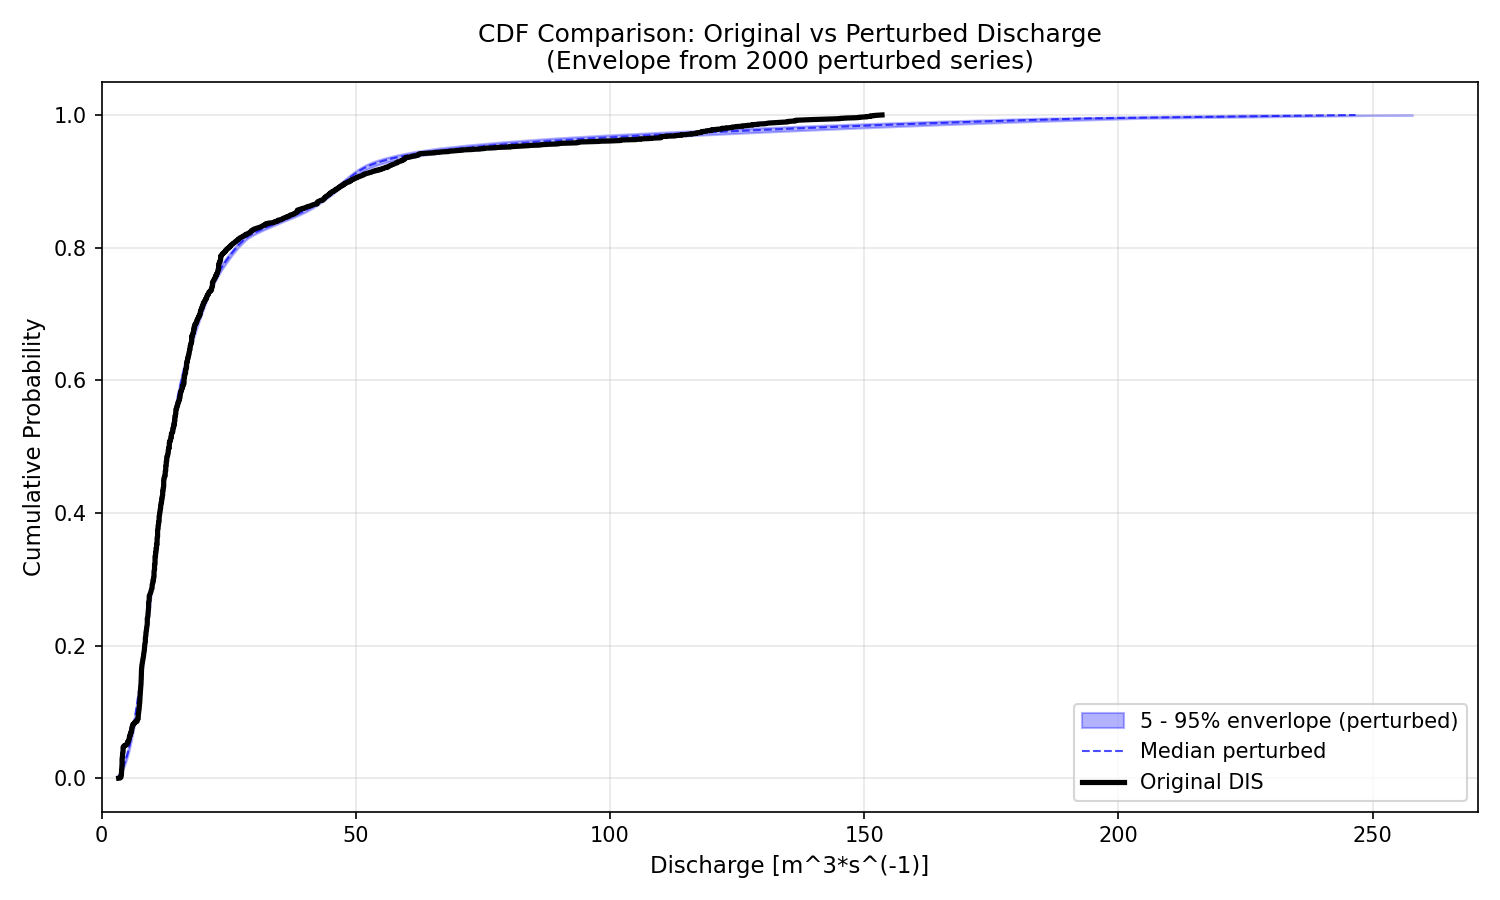
\includegraphics[width=\textwidth]{Figures/Ass_05/dis_cdf_comparison.png}
        \caption{cdf comparison}
        \label{fig:cdf}
    \end{minipage}
    \hfill
    \begin{minipage}[t]{0.48\textwidth}
        \centering
        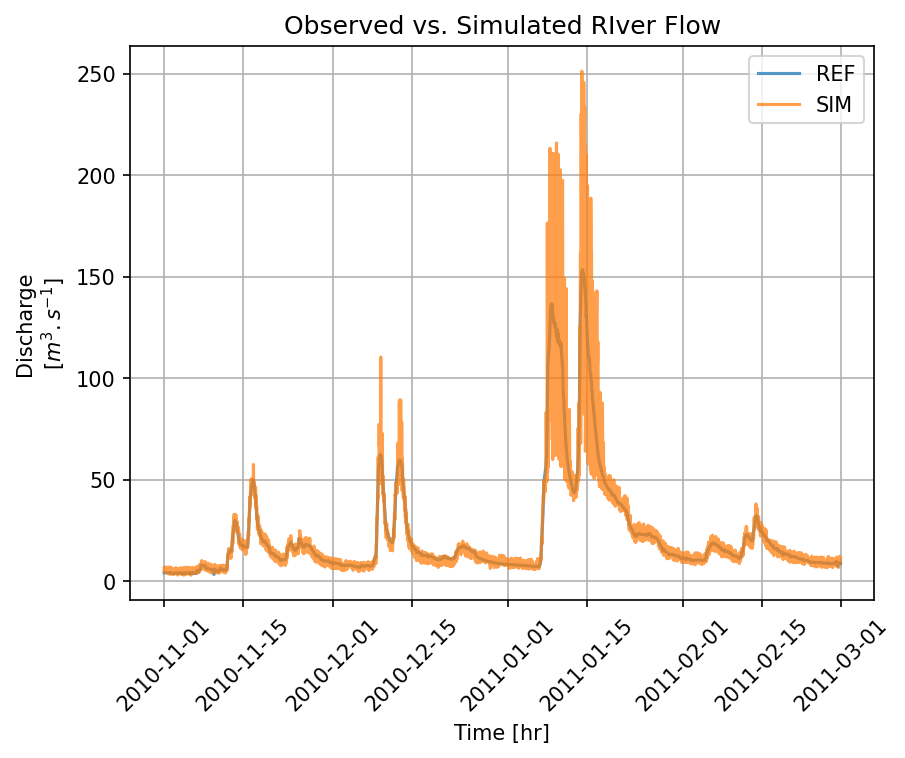
\includegraphics[width=\textwidth]{Figures/Ass_05/observed_vs_simulated_best_25.png}
        \caption{perturbed discharge example}
        \label{fig:pert_dis_eg}
    \end{minipage}
    %\caption{Development of OFV for each generation (right: zoom in)}
    %\label{dev_ofv_gen}
\end{figure}

For \SI{100}{\percent} of the perturbed series, without and with recalibration, the \ac{ofv} diminished (+0.1 to +0.18) (fig: \ref{fig: recal}, left and \ref{fig: dv_MP}). The recalibration resulted in an improvement rate of \SI{75.7}{\percent} (fig: \ref{fig: recal}, right), with an improvement around 0.0086. Thus, the negative effect of the change outweighs the small improvement, and the model cannot compensate for the output uncertainty. 

\begin{figure}[H]
    \centering
    \begin{minipage}[t]{0.48\textwidth}
        \centering
        
\includegraphics[width=\textwidth]{Figures/Ass_05/ofv_cdfs.png}
        %\caption{cdf}
        %\label{fig:cdf_recal}
    \end{minipage}
    \hfill
    \begin{minipage}[t]{0.48\textwidth}
        \centering
        
\includegraphics[width=\textwidth]{Figures/Ass_05/scatter_ofv_ref_vs_recalibrated.png}
        %\caption{perturbed discharge example}
        %\label{fig:pert_dis_eg}
    \end{minipage}
    \caption{comparing recalibration with no recalibration}
    \label{fig: recal}
\end{figure}

\begin{figure}[H]
\centering
  
\includegraphics[width=0.8 \textwidth]{Figures/Ass_05/scatter_ppt_change_vs_ofv.png}
    \caption{Development \ac{ofv} for 2000 perturbed series, left: with reference parameters, right: with recalibrated parameters}
    \label{fig: dv_MP}
\end{figure}

To evaluate each \ac{mp} separately, the \ac{cdf} for the 2000 recalibration is shown in figure \ref{fig: MP_cdf}, with the red line representing the reference parameter. Sensitive parameters are recognizable by a steep increase in the \ac{cdf}. Some of the most sensitive \ac{mp}, identified through the Sobol \ac{sa}, show minimal changes, close to zero. More unsensitive \ac{mp} have a slower increase over a larger range of the \ac{mp} range accordingly. Further, some of the \ac{mp} exhibit a step-like development, especially the threshold of the air temperature for snow (snw\_att). That is an indicator that the \ac{de} scheme converges to different solution areas despite the 600 generations. This also explains the broader range in the goodness-of-fit criterion. \\


Assignment 5 and \textcite{Wererberg.2022} both address uncertain discharge data in HBV calibration, but their approaches are fundamentally different. Assignment 5 is a diagnostic analysis: it perturbs the observed stage by ±15 cm, converts it to discharge using a fitted bipower rating curve, and evaluates the effect on calibration using the standard \ac{nse}-based objective function. This means the perturbed discharge series is treated as an exact observation, so the calibration remains uncertainty-blind. As a result, mean model performance drops substantially, with \ac{nse} decreasing from approximately 0.908 to 0.759, and recalibration recovers only 5.76\% of this loss. Westerberg et al. (2020), in contrast, use Bayesian MCMC to quantify rating-curve uncertainty, derive full per-time-step discharge uncertainty distributions, and include this uncertainty directly in a new flow-weighted objective function. Their main conclusion is that uncertainty should be embedded in the objective function itself, rather than handled by repeated calibration to many perturbed discharge realizations. Therefore, Assignment 5 demonstrates the impact of discharge uncertainty, whereas \textcite{Wererberg.2022} presents a more rigorous method for handling it during calibration.

\begin{figure}[H]
\centering
  
\includegraphics[width=1 \textwidth]{Figures/Ass_05/parameter_cdfs.png}
    \caption{Empirical CDF's of MP across 2000 recalibration runs}
    \label{fig: MP_cdf}
\end{figure}